\subsection{\texorpdfstring{\textcolor{red}{Steps 4--6: }}{Steps 4--6: }Peeling, terminal certification, and resources}
\label{app:upper-proof-structure}

The screen contract now yields the contraction in
\cref{main:eq:peeling-contraction} and sound stopping \textcolor{red}{in
\AlgoBlockNamedRef{peel}, certifying the graph in \AlgoBlockNamedRef{terminal}}.
We then count resources \textcolor{red}{across the complete sampler, including
\AlgoBlockNamedRef{centroid} and \AlgoGuardRef}, distinguishing
successful-path estimates from unconditional implementation caps.
\begin{example}[One peel commit, then two centroid batches]
\label{ex:algorithm-peel-centroids-20260918}
Let $\ResidualPositions=[15]$, $\DegreeCutoff=9$, and let the current
residual forest have edge set
\[
 E=\{\{1,i\}:2\le i\le9\}
   \cup\{\{1,10\},\{10,11\},\{11,12\},
          \{1,13\},\{13,14\},\{14,15\}\}.
\]
Vertex $1$ has degree $10$; every other vertex has degree at most $2$.
Suppose the reached screens are successful.  By
\AppLowDegreeScreenRef, $\ScreenRow{u}=\mathcal N_{\ResidualForest}(u)$
for $u\ne1$, whereas the row $\ScreenRow{1}$ need not be exact.
Nevertheless, \eqref{app:eq:claim-and-peel-set} gives
\begin{align*}
 \ClaimCount{1}
 &=\sum_{u\ne1}\mathbf1\{1\in\mathcal N_{\ResidualForest}(u)\}=10>9/2,\\
 \ClaimCount{v}
 &=|\mathcal N_{\ResidualForest}(v)\setminus\{1\}|
     +\mathbf1\{v\in\ScreenRow{1}\}
 \le2+1=3<9/2 \quad(v\ne1).
\end{align*}
Hence $\PeelSet=\{1\}$, regardless of the high-degree row's contents.
In \AlgoBlockRef{peel}, the sampler freezes this set and commits
vertex $1$ alone.  The residual
components are then
\[
 \{2\},\ldots,\{9\},\qquad
 10\text{--}11\text{--}12,\qquad 13\text{--}14\text{--}15.
\]
The next pass through \AlgoBlockRef{screen} uses the new history, before
the stopping test in \AlgoBlockRef{peel}.
Every residual degree is now at most $2$, so all its rows are exact.
Every incoming count is at most $2<9/2$, giving an empty peel set and
the exact terminal forest in \AlgoBlockRef{terminal}.
The successive batches of \AlgoBlockRef{centroid} are
\[
 B_1=\{2,\ldots,9,11,14\},\quad |B_1|=10,
 \qquad
 B_2=\{10,12,13,15\},\quad |B_2|=4.
\]
The eight isolates and the two path centers form $B_1$; deleting them
leaves the four singleton components in $B_2$.
Thus the example uses $1+2=3$ commit rounds.
This count excludes screen submissions and is not the total oracle depth.
\Cref{fig:algorithm-workflow-20260918} keeps the vertex positions fixed
throughout these steps.
\end{example}

\begin{figure}[H]
 \centering
 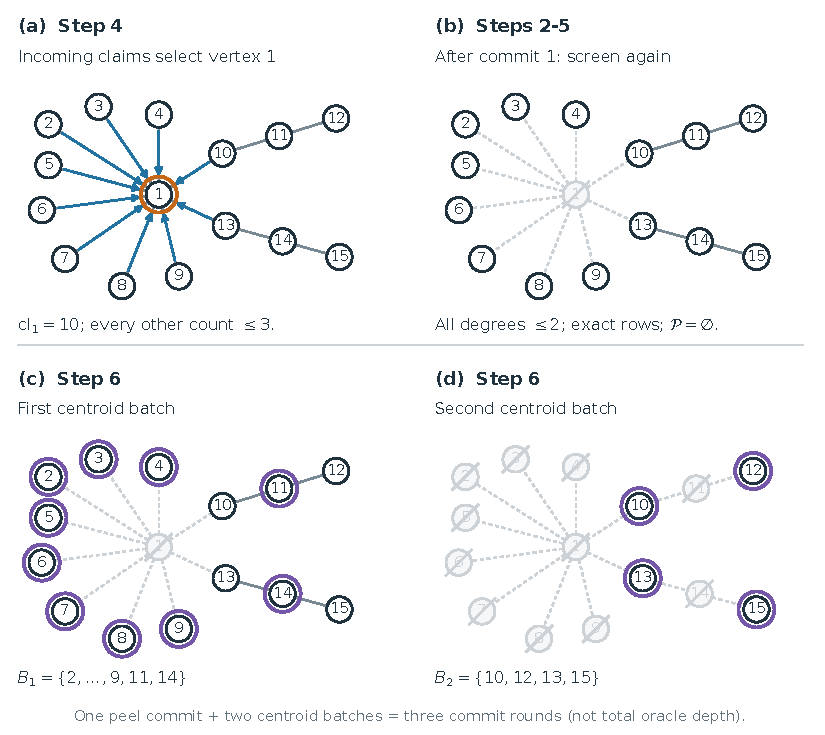
\includegraphics[width=\linewidth]{figures/algorithm_examples_2026-09-18/output/pdf/workflow_2026-09-18.pdf}
 \caption{The successful-screen path of
 \cref{ex:algorithm-peel-centroids-20260918}, with $N=15$ and $d=9$.
 Orange and violet rings denote the next peel or centroid commit;
 pale crossed vertices are already committed. The fills here are
 neutral, not random colors. The step labels refer to
 Algorithm~\ref{app:alg:complete-sampler}. A fresh screen separates (a) from (b);
 the terminal forest then needs no further discovery. All vertices
 remain individually visible.}
 \label{fig:algorithm-workflow-20260918}
\end{figure}


\paragraph{Intuition.}
A high-degree vertex that receives at most $\DegreeCutoff/2$ claims has
at most $\DegreeCutoff/2$ low-degree neighbors, because those neighbors
report it exactly.  It must therefore have more than $\DegreeCutoff/2$
neighbors inside the high-degree subforest.  A forest has fewer than
twice as many total degrees as vertices, so only a fraction at most
$4/\DegreeCutoff$ of high-degree vertices can survive one phase.
When $\DegreeCutoff=N^{\DegreeExponent+o(1)}$ with fixed
$\DegreeExponent>0$, the required number of phases is
$O_{\DegreeExponent}(1)$.

% Please keep this short statement together so its two stopping tests are visible.
\Needspace{12\baselineskip}
\begin{lemma}[Successful-path contraction and sound stopping\textcolor{red}{; \AlgoBlockRef{peel}, \AlgoBlockRef{terminal}}]
\label{app:lem:successful-path-structure}
Under the setup of Appendix~\ref{app:setup}, suppose preprocessing is feasible
and $\ScreenResolution<\EdgeSignal$.  Consider an execution path on which
every reached screen is successful in the sense of
\eqref{app:eq:screen-success-event}.  Let
$\HighDegreeCount{k}$ be the number of vertices whose residual degree exceeds
$\DegreeCutoff$ at the beginning of peel phase $k$.  After a nonempty peel
phase,
\begin{equation}
 \HighDegreeCount{k+1}
 \le\frac{4}{\DegreeCutoff}\HighDegreeCount{k},
 \label{app:eq:proof-peeling-contraction}
\end{equation}
with strict inequality whenever $\HighDegreeCount{k}>0$.
Moreover, either peel-loop stopping test in \AlgoBlockRef{peel} of
Algorithm~\ref{app:alg:complete-sampler}---an empty peel set or the
peel-phase cap---implies that the terminal residual
maximum degree is at most $\DegreeCutoff$.  The terminal certified graph is
therefore the true residual forest, so no cycle repair is performed.
\end{lemma}

\begin{proof}
\emph{1. High-degree neighbors of an unpeeled vertex.}
Fix a phase and define its high-degree set by
\begin{equation}
 \HighDegreeSet:=\{v\in\ResidualPositions:
                   d_{\ResidualForest}(v)>\DegreeCutoff\}.
 \label{app:eq:current-high-degree-set}
\end{equation}
At the beginning of phase $k$, $\HighDegreeCount{k}=|\HighDegreeSet|$.
Recall from \AlgoBlockNamedRef{peel} that the incoming claim count is
$\ClaimCount{v}=\sum_{u\in\ResidualPositions}\mathbf 1\{v\in\ScreenRow{u}\}$
and the peel threshold is $\ClaimCount{v}>\DegreeCutoff/2$.
For $v\in\HighDegreeSet\setminus\PeelSet$, every low-degree neighbor
reports $v$ exactly by \AppLowDegreeScreenRef.  Hence
\begin{align*}
 |\mathcal N_{\ResidualForest}(v)\setminus\HighDegreeSet|
 &=\sum_{u\in\ResidualPositions\setminus\HighDegreeSet}
       \mathbf 1\{v\in\mathcal N_{\ResidualForest}(u)\}\\
 &=\sum_{u\in\ResidualPositions\setminus\HighDegreeSet}
       \mathbf 1\{v\in\ScreenRow{u}\}
 \le\ClaimCount{v}\le\DegreeCutoff/2,\\
 d_{\ResidualForest[\HighDegreeSet]}(v)
 &=d_{\ResidualForest}(v)
       -|\mathcal N_{\ResidualForest}(v)\setminus\HighDegreeSet|\\
 &\ge d_{\ResidualForest}(v)-\ClaimCount{v}
 >\DegreeCutoff/2.
\end{align*}
The first equality uses the undirected nature of the forest.  Claims from
high-degree rows can only increase the incoming count, so they cannot
invalidate the bound for an unpeeled vertex.  We have shown that
\begin{equation}
 d_{\ResidualForest[\HighDegreeSet]}(v)
 >\frac{\DegreeCutoff}{2}.
 \label{app:eq:survivor-high-neighbors}
\end{equation}

\emph{2. Contraction after one peel phase.}
\emph{Empty survivor set.}
If $\HighDegreeSet\setminus\PeelSet=\emptyset$, no current high-degree vertex
survives the phase.  Deleting vertices cannot increase residual degrees, so
$\HighDegreeCount{k+1}=0$; this proves
\eqref{app:eq:proof-peeling-contraction}, strictly when
$\HighDegreeSet\ne\emptyset$.

\emph{Nonempty survivor set.}
Suppose instead that $\HighDegreeSet\setminus\PeelSet\ne\emptyset$.
Summing \eqref{app:eq:survivor-high-neighbors} over these unpeeled high-degree
vertices and using the forest degree-sum identity in
\cref{app:lem:forest-basics} gives
\begin{equation}
 \frac{\DegreeCutoff}{2}
 |\HighDegreeSet\setminus\PeelSet|
 <\sum_{v\in\HighDegreeSet\setminus\PeelSet}
   d_{\ResidualForest[\HighDegreeSet]}(v)
 \le2|E(\ResidualForest[\HighDegreeSet])|
 <2|\HighDegreeSet|.
 \label{app:eq:proof-high-degree-sum}
\end{equation}
Let $H'=(G',x_{G'})$ be the history after all singleton commits in the frozen
peel set of this phase, and recall the induced residual forest
$\ResidualForestAt{G'}=\TargetForest[\ResidualPositionsAt{G'}]$ from
\eqref{app:eq:history}.  Define
$\HighDegreeSetAt{H'}:=\{v\in\ResidualPositionsAt{G'}:
 d_{\ResidualForestAt{G'}}(v)>\DegreeCutoff\}$.
Deleting vertices cannot increase residual degrees:
\[
 \HighDegreeSetAt{H'}\subseteq\HighDegreeSet\setminus\PeelSet,
 \qquad
 \HighDegreeCount{k+1}=|\HighDegreeSetAt{H'}|
 \le|\HighDegreeSet\setminus\PeelSet|.
\]
Dividing \eqref{app:eq:proof-high-degree-sum} by $\DegreeCutoff/2$ now gives
$|\HighDegreeSet\setminus\PeelSet|<(4/\DegreeCutoff)|\HighDegreeSet|$,
and hence the strict form of \eqref{app:eq:proof-peeling-contraction}.  If
$\HighDegreeSet=\emptyset$, then the first case above gives equality
$\HighDegreeCount{k+1}=\HighDegreeCount{k}=0$.

\emph{3. Sound stopping at the phase cap.}
Initially, \cref{app:lem:forest-basics} makes the forest degree sum smaller
than $2N$, while each high-degree vertex has degree at least
$\DegreeCutoff+1$.  Hence
\begin{equation}
 \HighDegreeCount{0}<\frac{2N}{\DegreeCutoff+1}.
 \label{app:eq:initial-high-count}
\end{equation}
If the right-hand side is at most one, integrality already gives
$\HighDegreeCount{0}=0$.
Otherwise, once $\HighDegreeCount{k}=0$, deleting further vertices keeps every
later high-degree count equal to zero.  If this never occurs before the phase
cap, then $\HighDegreeCount{k}>0$ in every preceding phase, so the strict part
of \eqref{app:eq:proof-peeling-contraction} may be iterated.  In either case,
after $\PeelPhaseCap$ completed phases,
\begin{equation}
 \HighDegreeCount{\PeelPhaseCap}
 <\left(\frac4{\DegreeCutoff}\right)^{\PeelPhaseCap}
   \frac{2N}{\DegreeCutoff+1}
 \le
 \left(\frac8{\DegreeCutoff}\right)^{\PeelPhaseCap}
   \frac{2N}{\DegreeCutoff+1}
 \le1,
 \label{app:eq:phase-cap-eliminates-high-core}
\end{equation}
To check the last inequality, $\DegreeCutoff\ge9$ gives
$\log(\DegreeCutoff/8)>0$, and the ceiling in
\eqref{app:eq:phase-cap} gives
\begin{align*}
 \PeelPhaseCap\log(\DegreeCutoff/8)
 &\ge \PositivePart{\log(2N/(\DegreeCutoff+1))},\\
 \left(\frac8{\DegreeCutoff}\right)^{\PeelPhaseCap}
       \frac{2N}{\DegreeCutoff+1}
 &=\exp\!\left\{\log\frac{2N}{\DegreeCutoff+1}
                -\PeelPhaseCap\log(\DegreeCutoff/8)\right\}\le1.
\end{align*}
The integer in \eqref{app:eq:phase-cap-eliminates-high-core} is therefore zero.

\emph{4. Sound stopping with an empty peel set.}
If instead $\PeelSet=\emptyset$ while $\HighDegreeSet$ is nonempty, then
\eqref{app:eq:proof-high-degree-sum} holds with
$\HighDegreeSet\setminus\PeelSet=\HighDegreeSet$.  It would imply
$\DegreeCutoff/2<2$, contradicting $\DegreeCutoff\ge9$.  Hence an empty peel
set also certifies the absence of high-degree vertices.

\emph{5. \textcolor{red}{Bound peel-set size and certify the terminal graph.}}
We first check that the hard round cap cannot interrupt peeling.
\textcolor{red}{Fix a phase at history $\History$ with
$n:=|\ResidualPositions|\ge1$; if no vertex remains, the algorithm has
already returned.}
Low-degree exactness\textcolor{red}{~(\AppLowDegreeScreenRef)} and the row-size cap\textcolor{red}{~%
(\cref{app:def:row-selector})} imply
$|\ScreenRow{u}|\le d_{\ResidualForest}(u)$ for every $u$:
there is equality at low degree, while
$|\ScreenRow{u}|\le\DegreeCutoff<d_{\ResidualForest}(u)$ at high degree.
Counting each reported ordered pair once\textcolor{red}{, first at its
recipient and then in its reporting row,} gives
{\color{red}
\begin{align}
 \sum_{v\in\ResidualPositions}\ClaimCount{v}
 &=\sum_{v\in\ResidualPositions}\sum_{u\in\ResidualPositions}
       \mathbf 1\{v\in\ScreenRow{u}\}\notag\\
 &=\sum_{u\in\ResidualPositions}\sum_{v\in\ResidualPositions}
       \mathbf 1\{v\in\ScreenRow{u}\}\notag\\
 &=\sum_{u\in\ResidualPositions}|\ScreenRow{u}|\notag\\
 &\le\sum_{u\in\ResidualPositions}d_{\ResidualForest}(u)
 =2|E(\ResidualForest)|<2n.
 \label{app:eq:total-claim-bound}
\end{align}}
\textcolor{red}{The second equality interchanges finite sums; the last line
uses the forest degree sum in \cref{app:lem:forest-basics}.
Recall $\PeelSet=\{v\in\ResidualPositions:\ClaimCount{v}>\DegreeCutoff/2\}$
from \cref{app:eq:claim-and-peel-set}.
If $\PeelSet=\emptyset$, then $|\PeelSet|=0<4n/\DegreeCutoff$.
Otherwise its strict threshold gives}
{\color{red}
\begin{equation}
 \begin{aligned}
 \frac{\DegreeCutoff}{2}|\PeelSet|
 &<\sum_{v\in\PeelSet}\ClaimCount{v}
 \le\sum_{v\in\ResidualPositions}\ClaimCount{v}<2n,\\
 |\PeelSet|&<\frac{4n}{\DegreeCutoff}\le\frac{4N}{\DegreeCutoff}.
 \end{aligned}
 \label{app:eq:peel-set-size-proof}
\end{equation}}
\textcolor{red}{\AlgoBlockNamedRef{peel} freezes this set before its singleton
commits, so the phase uses exactly $|\PeelSet|$ rounds if completed and no
more if interrupted.}
With at most $\PeelPhaseCap$ phases, immediately before any planned peel
commit the completed-round counter satisfies
{\color{red}
\begin{equation}
 r<\frac{4N\PeelPhaseCap}{\DegreeCutoff}<\HardRoundCap-1,
 \label{app:eq:peel-before-hard-cap}
\end{equation}}
by \eqref{app:eq:screen-call-and-round-caps}.
\textcolor{red}{Thus \AlgoGuardRef\ cannot interrupt peeling.}
If all positions have already been committed, the residual graph is empty.
Otherwise peeling reaches one of the two tests identified in the statement.
Each pass executes \AlgoBlockRef{screen} before either stopping test
in \AlgoBlockRef{peel}.  At the
terminal history every residual vertex is consequently covered by
\AppLowDegreeScreenRef; the terminal screen is successful by
hypothesis, so all terminal rows are exact.  The
symmetrized edge set in \AlgoBlockNamedRef{terminal} is therefore
exactly $E(\ResidualForestAt{\star})$.  In particular, the cycle-repair loop
is skipped on the successful path.
\end{proof}

\begin{example}[A high-degree vertex can survive a peel phase]
\label{ex:algorithm-survivor-20260918}
This separate example illustrates the row contract used in
\cref{app:lem:successful-path-structure}, rather than specifying a
target--oracle pair.  Let $\DegreeCutoff=9$ and take the $65$ vertices
\[
 U=\{z\}\cup\{h_i:1\le i\le6\}
   \cup\{u_{i,j}:1\le i\le6,\ 1\le j\le9\}
   \cup\{s_1,s_2,s_3,s_4\},
\]
with edges
\[
 E=\{\{z,h_i\}:1\le i\le6\}
 \cup\{\{h_i,u_{i,j}\}:1\le i\le6,\ 1\le j\le9\}
 \cup\{\{z,s_j\}:1\le j\le4\}.
\]
At the history under consideration, take $\ResidualPositions=U$ and
$\ResidualForest=F=(U,E)$.
The center $z$ and all six hubs have degree $10$; all other vertices
are leaves.  Take the following row outputs, which obey the contract
\emph{exact at degree at most $d$, size at most $d$ elsewhere}:
\[
 \ScreenRow{z}=\ScreenRow{h_i}=\emptyset,\qquad
 \ScreenRow{u_{i,j}}=\{h_i\},\qquad
 \ScreenRow{s_j}=\{z\}.
\]
Computing the incoming counts, rather than reading a high-degree row's
size as its degree, gives
\begin{align*}
 \ClaimCount{z}&=4\le9/2, & \ClaimCount{h_i}&=9>9/2,\\
 \ClaimCount{u_{i,j}}&=\ClaimCount{s_j}=0,
 & \PeelSet&=\{h_1,\ldots,h_6\}.
\end{align*}
Thus $z$ is not peeled.  Before the commits its high-degree neighbors
are exactly $\{h_1,\ldots,h_6\}$, so their number is $6>9/2$, as required by
\eqref{app:eq:survivor-high-neighbors}.  After the six frozen singleton
commits in \AlgoBlockRef{peel}, its remaining neighbors are $\{s_1,\ldots,s_4\}$:
\begin{align*}
 d_{F[U\setminus\PeelSet]}(z)&=4,\\
 |\{v\in U:d_F(v)>9\}|&=7,\\
 |\{v\in U\setminus\PeelSet:d_{F[U\setminus\PeelSet]}(v)>9\}|&=0.
\end{align*}
The center survives as a vertex but ceases to be high-degree.
The $54$ hub leaves become isolated; none was committed in this phase.
\Cref{fig:algorithm-survivor-20260918} draws each of them separately.
\end{example}

\begin{figure}[H]
 \centering
 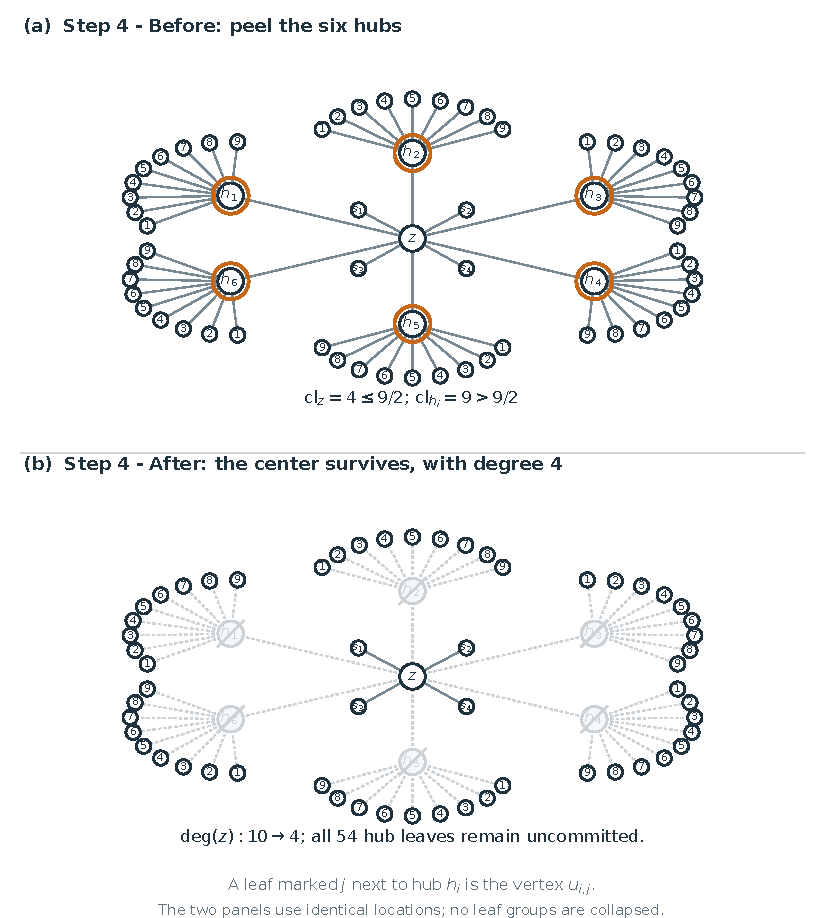
\includegraphics[width=\linewidth]{figures/algorithm_examples_2026-09-18/output/pdf/survivor_2026-09-18.pdf}
 \caption{The separate contraction example of
 \cref{ex:algorithm-survivor-20260918}. The six orange-ringed hubs are
 committed one at a time in \AlgoBlockRef{peel}, with no intervening screen or peel-set
 recomputation. Their $54$ leaves are drawn individually, not bundled.
 The unpeeled center $z$ changes from degree $10$ to degree $4$.
 The lower panel keeps the same locations and crosses out only the
 committed hubs.}
 \label{fig:algorithm-survivor-20260918}
\end{figure}


\paragraph{Intuition.}
\textcolor{red}{The total counterfactual-submission count is bounded by the
product of the screen-loop bounds:}
\[
 \textcolor{red}{\CounterfactualQueries\le}
 \underbrace{\ScreenColumnCount}_{\text{\textcolor{red}{source columns}}}\qquad
 \underbrace{\ScreenCallCap}_{\text{\textcolor{red}{screen calls}}}\qquad
 \underbrace{\RandomColoringCount}_{\text{\textcolor{red}{colorings/screen}}}\qquad
 \underbrace{\RandomColorCount}_{\text{source colors}}\qquad
 \underbrace{(\RandomColorCount+\ChunkCount)}_{\text{\textcolor{red}{chunks/coloring}}}.
\]
For rounds, \textcolor{red}{\cref{app:eq:peel-set-size-proof} bounds each peel set by}
$4N/\DegreeCutoff$; after the peel phases, centroid recursion needs only
$\lceil\log_2(N+1)\rceil$ layers.  The public cap extends the round bound to
failed-screen paths.  Total masked-state submissions, including
preprocessing and commits, are $\CounterfactualQueries+\CommitRounds+1$.

% Please keep the resource statement from starting with only two lines at a page foot.
\Needspace{14\baselineskip}
\begin{lemma}[Finite query and round counts\textcolor{red}{; \AlgoBlockRef{preprocess}--\AlgoBlockRef{centroid}}]
\label{app:lem:upper-resources}
Suppose preprocessing is feasible and
$\ScreenResolution<\EdgeSignal$.  On every execution path of
$\SelectedPackedSampler$ with any admissible row selector and the standard draft generator,
\begin{align}
 \CounterfactualQueries
 &\le\ScreenColumnCount\ScreenCallCap\RandomColoringCount
       \RandomColorCount(\RandomColorCount+\ChunkCount),
 \label{app:eq:proof-finite-Q}\\
 \CommitRounds
 &\le\HardRoundCap.
 \label{app:eq:proof-finite-R}
\end{align}
where
$\HardRoundCap=\lceil4N\PeelPhaseCap/\DegreeCutoff\rceil
+\lceil\log_2(N+1)\rceil+2$ is the public commit-round cap and
$\ScreenCallCap=\PeelPhaseCap+1$ is the screen-call cap from
\eqref{app:eq:screen-call-and-round-caps};
$\PeelPhaseCap$ is the peel-phase cap in \eqref{app:eq:phase-cap}.
In \eqref{app:eq:proof-finite-Q}, $\RandomColorCount$ and
$\RandomColoringCount$ are the fixed numbers of colors and independent
colorings per screen from \eqref{app:eq:random-color-parameters}.
The subscript $\mathrm{rnd}$ labels the randomized-color construction,
not a round index.
On a path on which every reached screen is successful, the sharper bound
\begin{equation}
 \CommitRounds
 <\frac{4N\PeelPhaseCap}{\DegreeCutoff}
   +\left\lceil\log_2(N+1)\right\rceil
 \label{app:eq:successful-path-rounds}
\end{equation}
holds, with no cycle repair or round-cap fallback.
The adaptive oracle depth, including the initial all-mask preprocessing
stage, satisfies
\begin{equation}
 \OracleDepth\le1+\CommitRounds+\ScreenCallCap.
 \label{app:eq:finite-oracle-depth}
\end{equation}
\end{lemma}

\begin{proof}

\emph{1. Count submissions over chunks, columns, and screens.}
Fix one screen execution at history $\History$.  Recall the quantities
counted in its loops:
\begin{itemize}
\item $\ScreenQueries$ denotes the number of masked-state submissions in
this one call to \AlgoBlockNamedRef{screen}, all made in
\AlgoBlockRef{probes}; preprocessing and commit submissions are excluded.
\item $\MaxBankSize=\max_{i\in\PositionSet}|\TokenBank{i}|$ is the largest
local vocabulary-bank size fixed in \cref{app:def:preprocessing}.
The number of submitted source columns is
$\ScreenColumnCount=\MaxBankSize+1$ when $\MaxBankSize\ge1$, and
$\ScreenColumnCount=0$ otherwise, as in \eqref{app:eq:screen-column-count}.
\item $\ColorCount=\RandomColorCount=8(\DegreeCutoff+1)$ is the number of
colors, and $\ColoringCount=\RandomColoringCount$ is the number of
independent colorings supplied by \AlgoBlockNamedRef{draft};
their choices are \eqref{app:eq:random-color-parameters}.
\item $\ChunkCount\in\PositionSet$ is the readout-chunk parameter from
\cref{app:algorithm-overview}: it sets
$\ReadoutChunkSize=\lceil N/\ChunkCount\rceil$, the maximum chunk size.
It is not the actual number of chunks.
\end{itemize}
For one coloring $\tau$, write $n_c:=|\ColorClass{\tau}{c}|$ and let
$\ChunksPerColoring{\tau}$ be the total number of readout chunks across
its color classes.  The deterministic partition
\eqref{app:eq:readout-chunks} in \AlgoBlockRef{chunks} creates exactly
$\lceil n_c/\ReadoutChunkSize\rceil$ chunks for every nonempty color class.
Therefore
\begin{align}
 \ChunksPerColoring{\tau}
 &=\sum_{c:n_c>0}
   \left\lceil\frac{n_c}{\ReadoutChunkSize}\right\rceil\notag\\
 &\le\sum_{c:n_c>0}
   \left(1+\frac{n_c}{\ReadoutChunkSize}\right)\notag\\
 &\le\ColorCount+\frac{|\ResidualPositions|}{\ReadoutChunkSize}
 \le\ColorCount+\ChunkCount.
 \label{app:eq:proof-chunk-count}
\end{align}
For each chunk, the bank columns and source-specific tail column in
\AlgoBlockRef{probes} use
$(\MaxBankSize+1)(\ColorCount-1)$ submissions.  When
$\MaxBankSize\ge1$, this is at most
$\ScreenColumnCount\ColorCount$.  Thus \AlgoBlockRef{chunks} supplies at
most $\ColorCount+\ChunkCount$ chunks per coloring, and
\AlgoBlockRef{probes} submits at most $\ScreenColumnCount\ColorCount$
states per chunk.  Summing over the $\ColoringCount$ colorings from
\AlgoBlockRef{draft} gives
\begin{equation}
 \ScreenQueries
 \le
 \underbrace{\ScreenColumnCount}_{\text{\textcolor{red}{source columns}}}\qquad
 \underbrace{\ColoringCount}_{\text{\textcolor{red}{colorings/screen}}}\qquad
 \underbrace{\ColorCount}_{\text{source colors}}\qquad
 \underbrace{(\ColorCount+\ChunkCount)}_{\text{chunks per coloring}}.
 \label{app:eq:proof-one-screen-count}
\end{equation}
When $\MaxBankSize=0$, the algorithm submits no screen state and both sides
are zero.  The screen runs initially and once after each of at most
$\PeelPhaseCap$ completed peel phases, hence at most $\ScreenCallCap$ times.
Substituting the randomized values of $\ColoringCount$ and $\ColorCount$
proves \eqref{app:eq:proof-finite-Q}.  The standard draft reuses preprocessing
and adds no query. Cycle repair runs no further screen: each singleton
repair is one commit submission, charged to $\CommitRounds$, not to
$\CounterfactualQueries$.

\emph{Returned oracle rows.}
For the standard zero-query draft, each counterfactual submission reads
only its chunk, of size at most $\ReadoutChunkSize=\lceil N/\ChunkCount\rceil$.
Preprocessing reads $N$ rows, and the disjoint commit batches
$B_1,\ldots,B_{\CommitRounds}$ partition $\PositionSet$
(\cref{app:def:admissible-algorithm}), so $\sum_{t=1}^{\CommitRounds}|B_t|=N$.
The main construction takes $\ChunkCount=\DegreeCutoff$.
Consequently the total number of returned oracle rows is at most
\[
 \underbrace{\lceil N/\ChunkCount\rceil\CounterfactualQueries}_{\text{screen submissions}}
 +\underbrace{N}_{\text{preprocessing}}
 +\underbrace{\sum_{t=1}^{\CommitRounds}|B_t|}_{\text{commits}}
 =\lceil N/\ChunkCount\rceil\CounterfactualQueries+2N.
\]


\emph{2. Count adaptive oracle stages.}
Once the history, draft, and colors are fixed, all submissions in a screen
can be issued in one parallel oracle stage \textcolor{red}{in
\AlgoBlockRef{probes}, because their states do not depend on replies from
that screen}.  Each commit requires one stage,
and preprocessing \textcolor{red}{in \AlgoBlockRef{preprocess}} requires one. This proves
\eqref{app:eq:finite-oracle-depth}.


\emph{3. Bound peeling rounds on a successful path.}
\textcolor{red}{On a path where every reached screen succeeds,
\eqref{app:eq:peel-set-size-proof} in
\cref{app:lem:successful-path-structure} shows that every nonempty peel phase in
\AlgoBlockNamedRef{peel} commits fewer than $4N/\DegreeCutoff$ vertices,
one per round.  At most $\PeelPhaseCap$ such phases therefore use fewer than
$4N\PeelPhaseCap/\DegreeCutoff$ rounds.
The bound \eqref{app:eq:peel-before-hard-cap} also shows that
\AlgoGuardRef\ cannot interrupt these commits.}


\emph{4. Bound terminal centroid rounds and exclude repair and fallback.}
By Lemma~\ref{app:lem:successful-path-structure}, the terminal certified graph
is the true residual forest.  Lemma~\ref{app:lem:residual-markov} makes its
connected components conditionally independent.  At any layer of
\AlgoBlockNamedRef{centroid}, let
the current components be $T_1,\ldots,T_m$, with selected centroids
$\ComponentCentroid{1},\ldots,\ComponentCentroid{m}$, and set
$B=\{\ComponentCentroid{1},\ldots,\ComponentCentroid{m}\}$.  Then
\begin{equation}
 \TargetLaw(X_B=x_B\mid X_G=x_G)
 =\prod_{\ell=1}^m
   \TargetLaw\bigl(X_{\ComponentCentroid{\ell}}
   =x_{\ComponentCentroid{\ell}}\mid X_G=x_G\bigr).
 \label{app:eq:centroid-batch-factorization}
\end{equation}
Thus their exact singleton rows define the exact joint batch conditional.
By
\cref{app:lem:forest-basics}, removing a centroid leaves components of size at
most half the parent size, so after
$\ell$ terminal batches every remaining component has size at most $N/2^\ell$.
For $\ell=\lceil\log_2(N+1)\rceil$ this is smaller than one.  Adding the peeling
and terminal rounds proves \eqref{app:eq:successful-path-rounds}.  Its
right-hand side is smaller than $\HardRoundCap-1$ by
\eqref{app:eq:screen-call-and-round-caps}; hence the hard-cap check is never
triggered during the terminal stage either. The terminal graph is already
a forest, so the cycle-repair loop adds no rounds.


\emph{5. Enforce the round cap on every path.}
It remains to verify the unconditional randomized round bound enforced by
\AlgoGuardRef. Initially $r=0\le\HardRoundCap-1$. Before every peel, repair,
or centroid commit, the algorithm checks whether $r=\HardRoundCap-1$.
If equality holds, it commits all remaining positions in the reserved
final round and returns. Otherwise the integer counter satisfies
$r\le\HardRoundCap-2$, and the next commit leaves
$r+1\le\HardRoundCap-1$.
Every such commit is nonempty and irrevocable, so it removes at least
one remaining position; cycle repair cannot continue indefinitely.
If it ends without the cap fallback, the remaining working graph is a
forest and centroid completion applies. Induction over commit operations
therefore gives $\CommitRounds\le\HardRoundCap$ on every path, proving
\eqref{app:eq:proof-finite-R}.
\end{proof}
